%%%%%%%%%%%%%%%%%%%%%%%%%%% asme2ej.tex %%%%%%%%%%%%%%%%%%%%%%%%%%%%%%%
% Template for producing ASME-format journal articles using LaTeX    %
% Written by   Harry H. Cheng, Professor and Director                %
%              Integration Engineering Laboratory                    %
%              Department of Mechanical and Aeronautical Engineering %
%              University of California                              %
%              Davis, CA 95616                                       %
%              Tel: (530) 752-5020 (office)                          %
%                   (530) 752-1028 (lab)                             %
%              Fax: (530) 752-4158                                   %
%              Email: hhcheng@ucdavis.edu                            %
%              WWW:   http://iel.ucdavis.edu/people/cheng.html       %
%              May 7, 1994                                           %
% Modified: February 16, 2001 by Harry H. Cheng                      %
% Modified: January  01, 2003 by Geoffrey R. Shiflett                %
% Use at your own risk, send complaints to /dev/null                 %
%%%%%%%%%%%%%%%%%%%%%%%%%%%%%%%%%%%%%%%%%%%%%%%%%%%%%%%%%%%%%%%%%%%%%%

%%% use twocolumn and 10pt options with the asme2ej format
\documentclass[twocolumn,10pt]{asme2ej}

\usepackage{graphicx}
\usepackage{amssymb}
\usepackage{amsmath}
\usepackage{float}
%\usepackage[section]{placeins}
%\usepackage[below]{placeins}
\usepackage{epstopdf}
\usepackage{hyperref}
\usepackage{breakurl}
%\DeclareGraphicsRule{.tif}{png}{.png}{`convert #1 `dirname #1`/`basename #1 .tif`.png}
\newcommand\bslash{\char`\\}
\newcommand\lt{\char`\<}
\newcommand\gt{\char`\>}
\newcommand{\supers}[1]{\ensuremath{^\textrm{{\scriptsize #1}}}}
\newcommand{\subs}[1]{\ensuremath{_\textrm{{\scriptsize #1}}}}

%% The class has several options
%  onecolumn/twocolumn - format for one or two columns per page
%  10pt/11pt/12pt - use 10, 11, or 12 point font
%  oneside/twoside - format for oneside/twosided printing
%  final/draft - format for final/draft copy
%  cleanfoot - take out copyright info in footer leave page number
%  cleanhead - take out the conference banner on the title page
%  titlepage/notitlepage - put in titlepage or leave out titlepage
%  
%% The default is oneside, onecolumn, 10pt, final


\title{Assessment of 3D Shading Calculations for Photovoltaic System Modeling}

%%% first author
\author{Aron P. Dobos
    \affiliation{
	Senior Engineer, NREL\\
	aron.dobos@nrel.gov
    }	
}
\author{Janine M. Freeman
    \affiliation{
	Energy Modeling Engineer, NREL\\
	janine.freeman@nrel.gov
    }	
}
\author{Nicholas A. DiOrio
    \affiliation{
	Modeling and Software Engineer, NREL\\
	nicholas.diorio@nrel.gov
    }	
}

\begin{document}

\maketitle    

%%%%%%%%%%%%%%%%%%%%%%%%%%%%%%%%%%%%%%%%%%%%%%%%%%%%%%%%%%%%%%%%%%%%%%
\begin{abstract}
{\it 
This paper assesses three popular models for estimating shading losses on photovoltaic systems.  Several hypothetical and actual scenes are used to compare the loss predictions of the three dimensional (3D) shading calculators in the System Advisor Model (SAM), PVsyst, and PV*SOL tools.   Comparisons with measured shade blocking from a SunEye device are also made for five actual systems.  Results show some notable differences in hourly shade loss profiles among the studied tools, even for very simplistic geometries.  However, on a annual energy basis, the differences appear to cancel out to some degree and result in errors that are comparable to documented variations in energy predictions.   These outcomes demonstrate a need for further development and improvement of 3D shade calculators to reduce model prediction errors and variability.
}
\end{abstract}

%%%%%%%%%%%%%%%%%%%%%%%%%%%%%%%%%%%%%%%%%%%%%%%%%%%%%%%%%%%%%%%%%%%%%%
\section{Introduction}

Major reductions in the cost of photovoltaic (PV) systems in the past several years have led to a proliferation of PV deployments at all market scales.  Particularly for distributed systems, which are frequently installed on existing rooftops in an urban environment, shading from nearby obstructions (other buildings, trees, etc) can have a major impact on energy production.  However, as such losses in available irradiance may no longer banish a system from economic viability, it becomes imperative to have accurate software tools to model shading losses in a 3D environment.  

Several tools for shade impact assessment exist on the market.  Common hardware include the SunEye ~\cite{suneye} and SolarPathfinder ~\cite{solarpathfinder} devices that require a site visit and potentially scaling of the rooftop itself to take pictures skydome blocking pictures that are subsequently processed by special software to estimate solar access at the proposed installation site.  Reducing assessment, siting, permitting, and other so-called balance of system (BOS) costs often pushes solar vendors to minimize site visits and thus the need for accurate 3D modeling of shade loss becomes evident.  Possible methods include Light Detection and Ranging (LiDAR) analysis~\cite{jakubiec2013}, topographical assessment using geospatial information systems (GIS)~\cite{melius2013}, and of course 3D modeling in computer-aided design (CAD) software which is the subject of this present assessment.

Commonly used desktop software for photovoltaic system performance estimation include PVsyst~\cite{pvsyst}, PV*SOL~\cite{pvsol}, and NREL's System Advisor Model (SAM)~\cite{sam}.  More recent additions to these offerings include Helioscope~\cite{helioscope}, PV Complete~\cite{pvcomplete}, and others.  All of these tools propose estimate shading impacts by calculating the portion of a PV panel whose view of the sun is blocked by nearby obstructions at various times of the year.  Each software includes an interactive user interface for laying out PV panels in 3D space, adding obstructions such as trees, telephone poles, angled roof segments, and other geometric features.  Once the scene is specified, standard computer graphics techniques or ray tracing methods are used to determine the PV panel shade area fractions as the entire scene is transformed by rotation to mimic the movement of the sun over the horizon.

To date, published comparisons and validation of PV performance modeling tools has focused on energy production in well characterized systems without irregular obstruction shading~\cite{blair2013,freeman2013,freeman2014,haroon2012,yates2010}.  In general, the collective data in these works indicate that most PV performance models, using typical assumptions for soiling and other losses, yield predictions within roughly $\pm$~5~\% of measured system performance.  However, to date, the accuracy of 3D shading loss calculations has not been independently verified.  In addition, one would expect shading loss predictions from all software tools to match very closely if not identically, as the linear shaded area calculations stem solely from geometric considerations.  Furthermore, the sensitivity of estimated shade loss and impact on annual energy production to the accuracy of the 3D model itself remains unknown.

We investigate these issues using SAM, PVsyst, and PV*SOL to assess and better understand any differences in modeled shade loss among the three tools and provide a basis for further model improvement.  First, the procedure in SAM for calculating 3D shading losses is presented as a representative example.  Next, three extremely simple geometries are considered to quantify intermodel differences in shade loss profiles, followed by four systems accompanied by SunEye site measurements are assessed.  Finally, we consider the sensitivity of modeled energy predictions to errors in defining the 3D scene before wrapping up with some brief concluding remarks.

\section{Methodology -- need to rewrite: currently based on tech manual text, this a placeholder really...}

The SAM 3D shade calculator calculates a set of beam and diffuse shade factors from a three-dimensional representation of the photovoltaic array and nearby shading objects.  Objects in the 3D scene are represented by a set of polygons whose coordinates are specified in 3D space (x,y,z).  Polygons associated with the photovoltaic array or modules are marked as ``active surfaces'', so that the calculator can determine for which surfaces shading and blocking should be evaluated.  The geometry system uses a right-handed coordinate system in which $+x$ points east, $+y$ points north, and $+z$ points normal out of the ground towards the sky. 

\subsection{Beam Shading Loss}

The calculation procedure for linear shading losses for each active surface at each time step is as follows:

\begin{enumerate}
\item Calculate the solar zenith and azimuth angles for the current time stamp (month, day, hour, minute) and location (latitude, longitude, time zone).
\item Create a list of polygons from the scene objects in untransformed 3D space.
\item Calculate the axis $x$, $y$, and $z$ rotation angles corresponding to a rotation of the scene associated with the current sun position.  In other words, the 3D scene is rotated so that it is shown as if it were observed from the sun.
\item Using this 3D rotation matrix, calculate the rotated coordinates of each polygon vertex to transform the whole scene into the line of sight from the sun using a parallel projection.  This assumes the sun is infinitely far away and that the sun rays reaching the scene are essentially parallel to one another.
\item Using a backface culling algorithm, eliminate polygons from the scene that face away from the sun and are not visible.
\item Apply the binary space partitioning (BSP) algorithm to sort all the remaining visible polygons in back-to-front order.  Polygons at the ``front'' are closest to the sun.
\item Discard the transformed $z$ coordinate to effectively ``flatten'' the scene into two dimensions, as if it were viewed from the infinitely far away sun.
	\item For each active surface:
	\begin{enumerate}
	\item Create a list of polygons (regular and other active surfaces) that are in front of the active surface, that is, between it and the sun.
	\item Using a 2D polygon clipping algorithm, determine the intersection between the active surface and the list of potential blocking polygons.
	\item The resulting intersection polygon's area divided by the active surface polygon area gives the linear shading fraction for that active surface at the current time (sun position).
	\end{enumerate}
\item If subarrays and strings are specified, determine the appropriate shade fractions for each piece from the sum total of the intersected (shaded) areas divided by the sum total of the unshaded active surface areas associated with each string or subarray.   If no strings or subarrays are specified in the geometry, the total intersected (shaded) area divided by the total unshaded active surface area is reported as the overall average shading fraction.
\end{enumerate}



\subsection{Sky Diffuse Blocking}

The 3D shading calculator also estimates the loss of available diffuse irradiance to the active photovoltaic surfaces due to blocking of the sky dome by obstructions.  The procedure is as follows:
\begin{enumerate}
\item Divide the hemispherical sky dome into sections of some number of azimuth and zenith angle divisions.  By default, SAM uses 1 degree increments in both directions, for a total of 360 * 90 = 32400 divisions.
\item For each position, transform the scene to the solar azimuth and zenith angle.
\item Calculate the intersected (shaded) areas on each active surface polygon using the same procedure as for the beam irradiance shading loss.
\item Integrate the shade loss over all positions in the sky dome by multiplying the observed shaded fraction with the solid angle of spherical integration $\sin(\theta_z)$.  This accounts for the fact that the sky dome divisions at the top of the hemisphere are much smaller than near $\theta_z\approx 0$.
\end{enumerate}

This procedure results in an estimate of the view factor of the active surfaces in each subarray to the sky dome, and hence the effective diffuse irradiance loss.  The model assumes an isotropic diffuse sky, and does not adjust for increased circumsolar diffuse irradiance.


\section{Assessment of Simple Geometries}

The purpose of this investigation is to isolate and identify any differences in the geometrical calculations for shaded area performed by the three models considered in this paper.  Three very simple but well-defined geometries were created in three locations to simultaneously test a selection of orientations, dimensions, and locations in the world.  These scenes are shown in Fig.~\ref{fig:scene1}-\ref{fig:scene3}, with location information given in Table~\ref{tab:locations}.

\begin{table}[h!]
\begin{center}
\begin{tabular}{lccc}
Location & Latitude & Longitude & Time zone \\
\hline
Denver, Colorado & 39.73 & -104.99 & -7 \\
Quito, Ecuador & -0.18 & -78.46 & -5 \\
Perth, Australia & -31.95 & 115.85 & 8 \\
\end{tabular}
\caption{Locations of prototypical 3D geometries.}
\label{tab:locations}
\end{center}
\end{table}


\begin{figure}[h!]
\begin{center}
\resizebox{2.75in}{!}{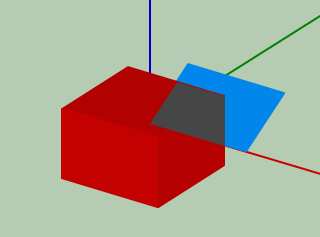
\includegraphics{scene1.png}}
\end{center}
\caption{Simple scene in Denver, Colorado.}
\label{fig:scene1}
\end{figure}

\begin{figure}[h!]
\begin{center}
\resizebox{2.75in}{!}{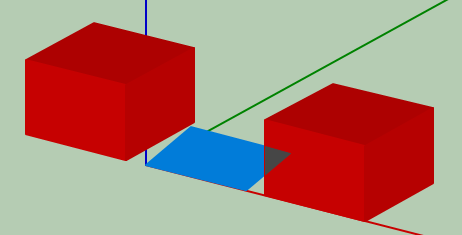
\includegraphics{scene2.png}}
\end{center}
\caption{Simple scene in Quito, Ecuador.}
\label{fig:scene2}
\end{figure}

\begin{figure}[h!]
\begin{center}
\resizebox{2.75in}{!}{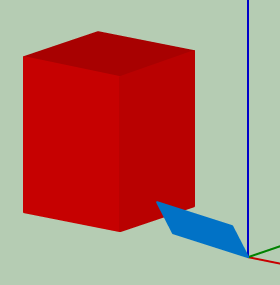
\includegraphics{scene3.png}}
\end{center}
\caption{Simple scene in Perth, Australia.}
\label{fig:scene3}
\end{figure}

After entered each scenario manually into SAM, PVsyst, and PV*SOL using each tool's interactive 3D scene editor, simulation results were exported and post processed to extract the hourly beam irradiance shading loss.  This data is readily provided by SAM's 3D shading calculator when used in the time series analysis mode.  For PVsyst, the hourly data is given as a shade fraction from 0 (completely shaded) to 1 (unshaded) in the \texttt{FShdBm} data column. 

Making a comparison with PV*SOL results is somewhat more complicated.  PV*SOL does not directly provide a shaded fraction or similar output, and so the shading loss must be recovered from other data.  Horizon shading effects that reduce the diffuse irradiance are first deducted from the total irradiance available to the modules, and this amount is then converted into a ``rated'' or nominal PV DC output.  Then, the difference between nominal DC output power in kilowatt-hours and shaded DC output power in the same units can be used to recover an estimate for the beam shading fraction alone.  First, we estimate the DC power loss from horizon shading $L_h$ (kWh) at each our using the module's standard test condition (STC) efficiency:
\begin{equation}\label{eqn:pvsol_lh}
L_h = L_{i,0} A \eta
\end{equation}
where $L_{i,0}$ is the provided horizon irradiance loss in Watts/m$^2$, $A$ is the module area, and $\eta$ the STC efficiency.  Then, the loss due to shadowing from obstructions may be retrieved at each hour:
\begin{equation}\label{eqn:pvsol_ls}
L_s (\%) = 100 \cdot \frac{ M_{dc} + L_h }{ M_{0} + L_h }
\end{equation}
where $M_{dc}$ is the shaded module energy (kWh) and $M_0$ is the rated PV DC output.


Geometric shading loss for the three prototypical scenarios are shown in Fig.~\ref{fig:simple_denver}-\ref{fig:simple_perth} for four representative days of the year.  SAM and PVsyst estimate nearly identical shading losses but for some occasional deviations that are rather minor in magnitude at sun-up and sun-down hours for Denver and Quito.  These deviations may result from small differences in the sun position calculation algorithms used by the tools, and the assumptions in each for how to handle hours in which the sun is only partially above the horizon.  Although good agreement persists for Perth, PVsyst predicts a much more pronounced shade loss around hours 18-19 in January, April, and October than SAM, but only in that single hour of the day.  One might presume that running these shade loss calculations at subhourly timesteps may recover finer detail of the actual shading profiles, which may explain some of these differences.  We note that currently only SAM offers subhourly shade loss calculations, and \textbf{so subsequent exploration of time step effects will be limited to SAM}.

We also observe more frequent and more varied divergences in the PV*SOL's estimates of shading loss.  Although the daily profiles agree fairly well in a qualitative sense for Denver, the Quito and Perth scenarios show significant differences.  Differences seem to be greatest at the beginning and end of the day, and in some cases, such as on April 1st in Quito, over a 50~\% absolute difference in shade loss for several hours in the day.  PV*SOL shows better agreement with SAM and PVsyst before hour 15, after which it predicts much greater shading losses.  The reasons for these differences are not immediately clear.  Even if the post-processing procedure described previously is not perfect, one would expect differences in absolute magnitude but still a consistent shape to the loss profile.   We would emphasize again, though, that in theory all three modules should predict identical geometric shading losses for these well-characterized prototypical scenarios.  \textbf{Further effort to find out cause of these differences is needed}

\begin{figure*}[h!]
\begin{center}
\scalebox{0.55}{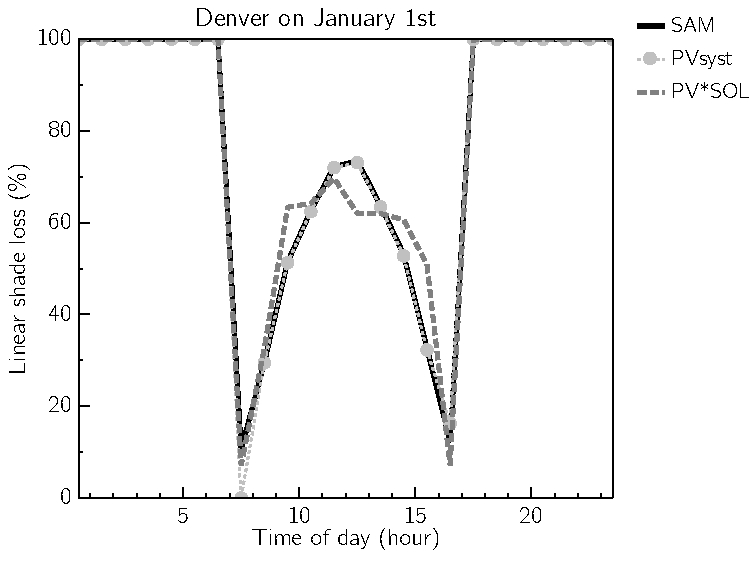
\includegraphics{denver_1.pdf}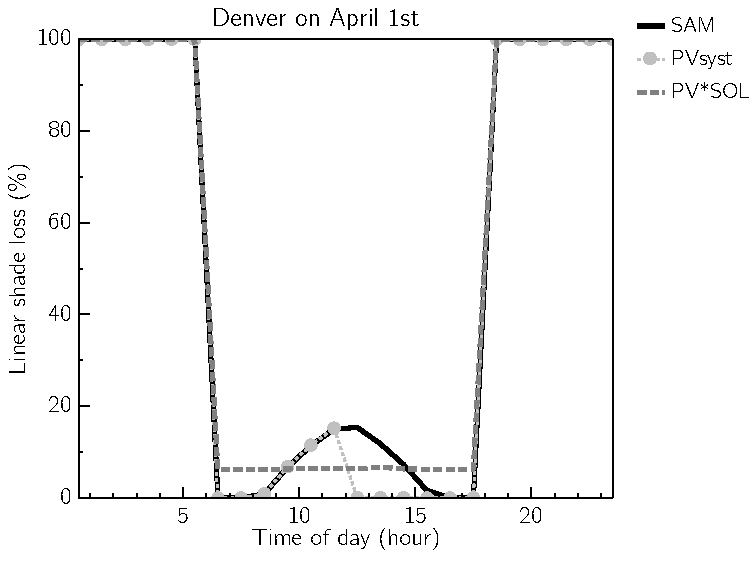
\includegraphics{denver_2.pdf}}
\scalebox{0.55}{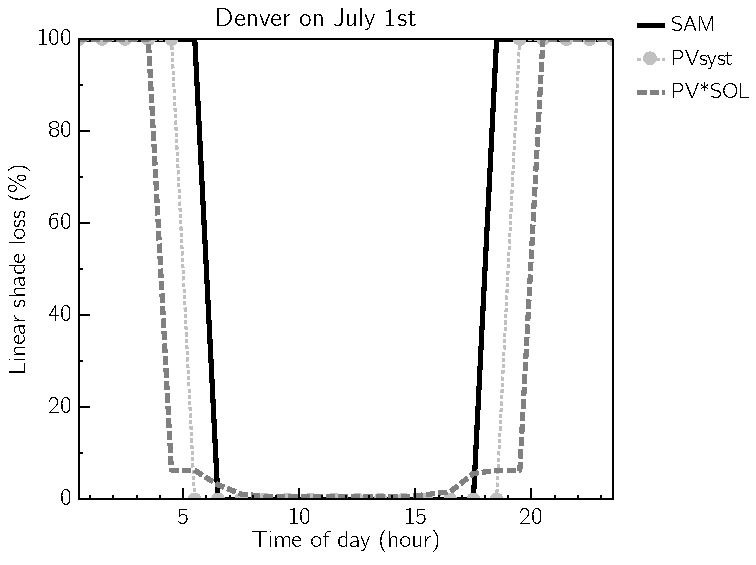
\includegraphics{denver_3.pdf}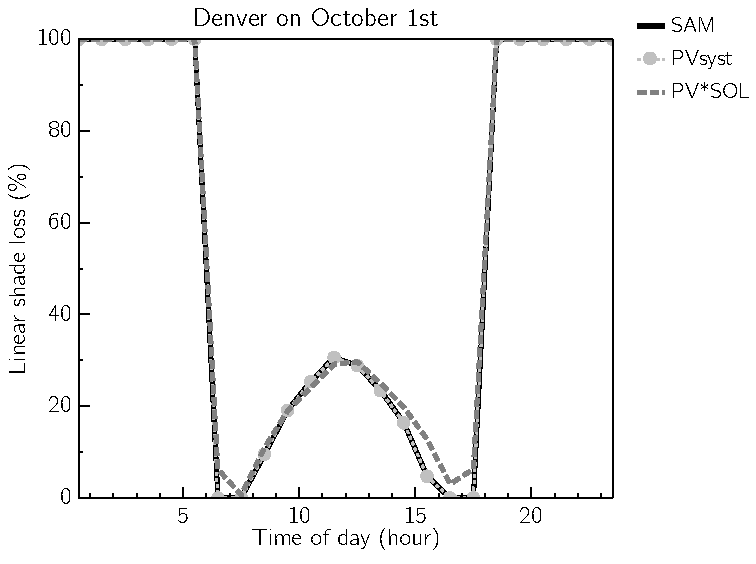
\includegraphics{denver_4.pdf}}
\end{center}
\caption{Daily shade loss profiles for a prototypical system Denver, Colorado.}
\label{fig:simple_denver}
\end{figure*}

\begin{figure*}[h!]
\begin{center}
\scalebox{0.55}{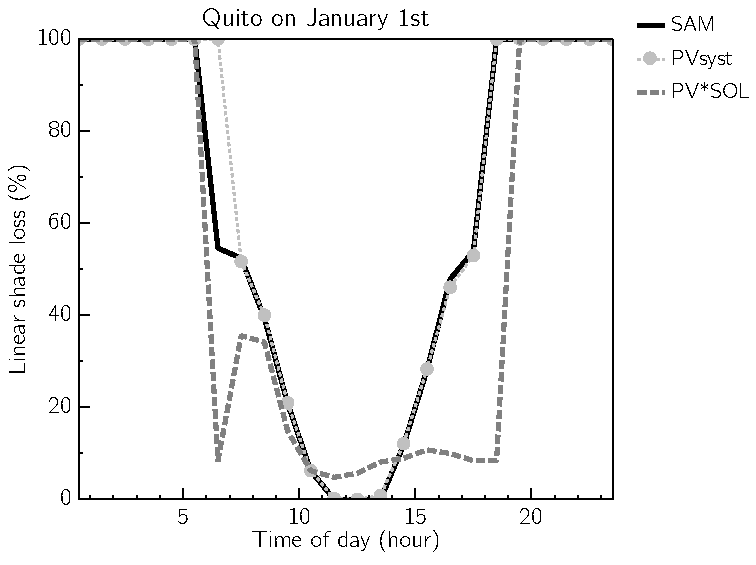
\includegraphics{quito_1.pdf}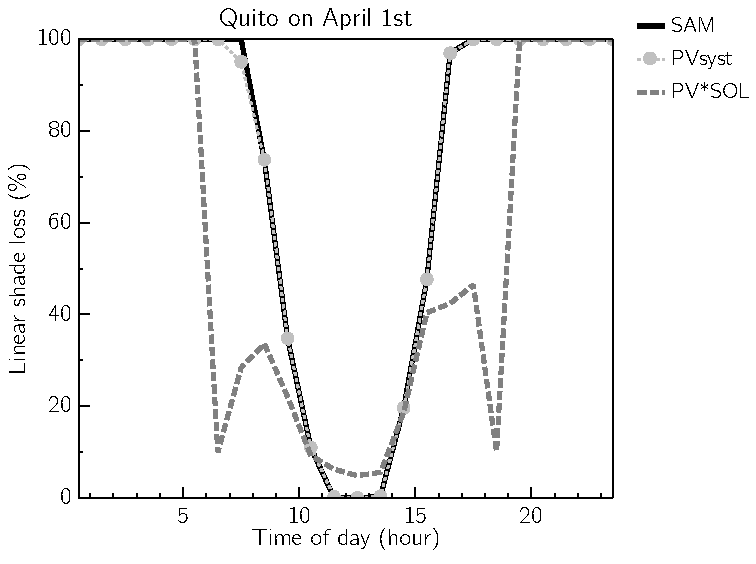
\includegraphics{quito_2.pdf}}
\scalebox{0.55}{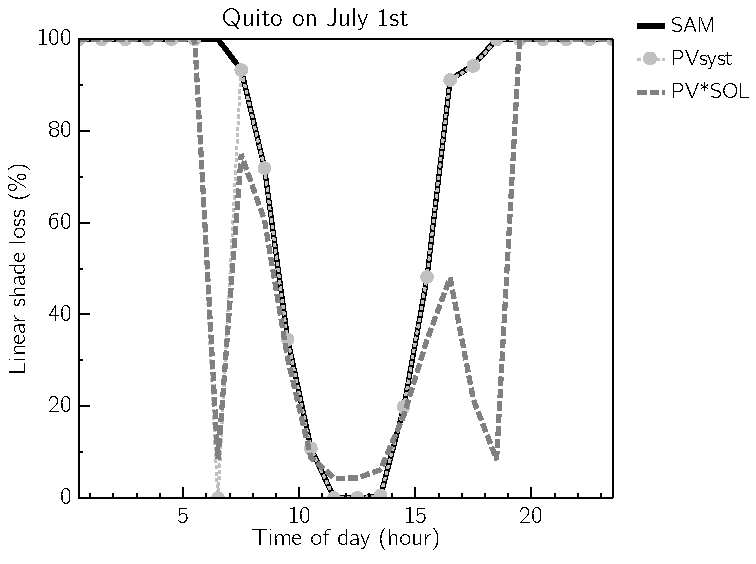
\includegraphics{quito_3.pdf}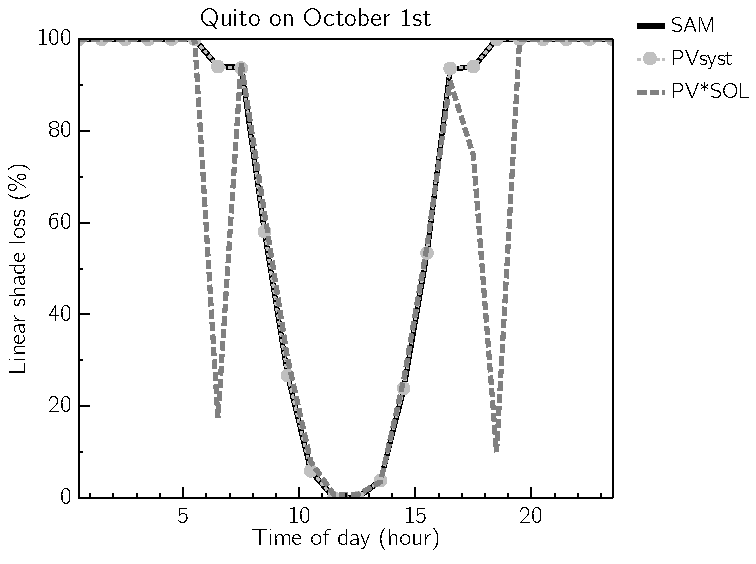
\includegraphics{quito_4.pdf}}
\end{center}
\caption{Daily shade loss profiles for a prototypical system Quito, Ecuador.}
\label{fig:simple_quito}
\end{figure*}


\begin{figure*}[h!]
\begin{center}
\scalebox{0.55}{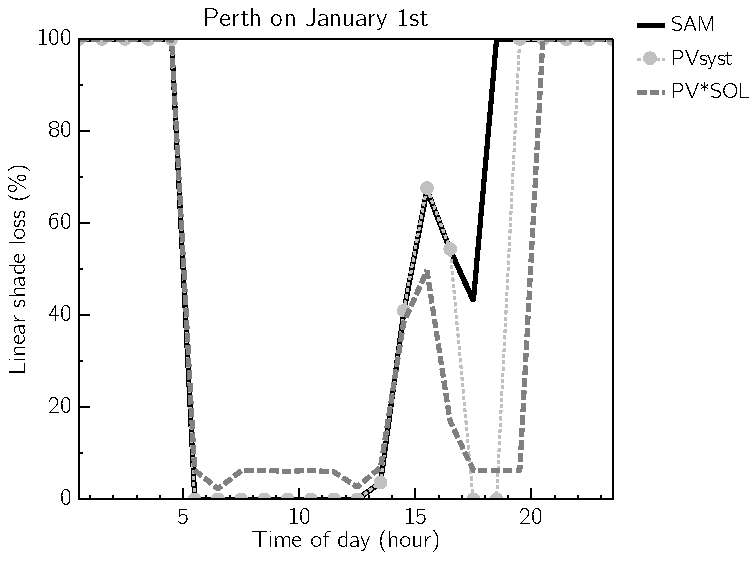
\includegraphics{perth_1.pdf}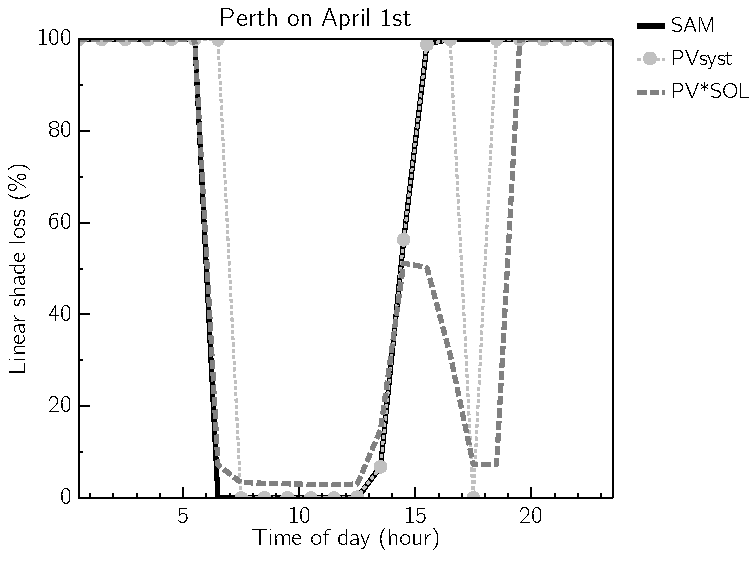
\includegraphics{perth_2.pdf}}
\scalebox{0.55}{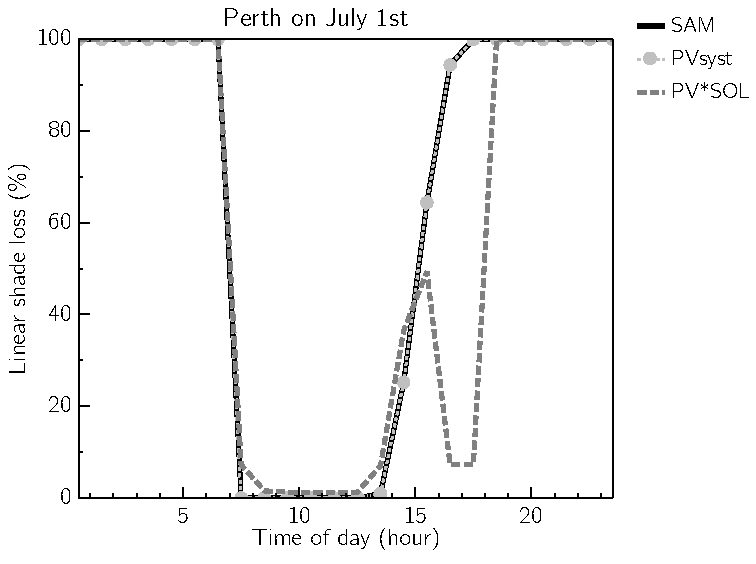
\includegraphics{perth_3.pdf}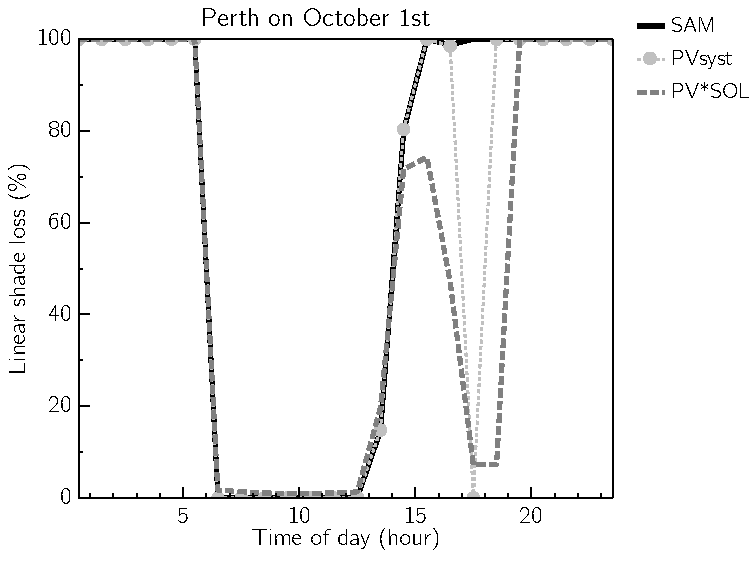
\includegraphics{perth_4.pdf}}
\end{center}
\caption{Daily shade loss profiles for a prototypical system Perth, Australia.}
\label{fig:simple_perth}
\end{figure*}


In addition to beam irradiance shading losses arising from obstructions blocking the sun rays to the PV array, obstructions also reduce the effective portion of the sky dome visible to the array.  Conservatively assuming an isotropic diffuse sky, the available diffuse irradiance is reduced by the view factor of the PV array to the sky, and remains constant through the year as the sun position does not affect the available sky diffuse.  Estimated diffuse shading loss for the three scenarios are listed in Table.~\ref{tab:diffuse_loss}.

\begin{table}[h!]
\begin{center}
\begin{tabular}{lccc}
Scene & SAM & PVsyst & PV*SOL \\
\hline
Denver & 8.8~\% & 18.5~\% & ? \\
Quito  & 16.8~\% & 18.1~\% & ? \\
Perth  & 8.1~\% & 8.6~\% & ? \\
\end{tabular}
\caption{Sky diffuse loss estimates for prototypical systems.}
\label{tab:diffuse_loss}
\end{center}
\end{table}

SAM and PVsyst estimate similar diffuse loss in Quito and Perth, but PVsyst estimates over double the diffuse loss for the Denver scenario.  The reason for this behavior is not clear.  \textbf{PV*SOL needs diffuse loss breakout}



\section{Comparison with On-site Measurements}

In this section, we apply the same procedures to four actual systems for which monthly solar access estimates have been measured using SunEye or SolarPathfinder devices.  The system names and locations are listed in Table~\ref{tab:measured_system_names}.  This analysis does not purport to have the modeled 3D geometry of the roofs, trees, and PV systems impeccably reflect reality - but rather to be a ``reasonable'' model for each scene.  Each scene was first entered into the SAM shading tool (Figs.~\ref{fig:ivanhoe}-\ref{fig:paradise}, and then subsequently rebuilt in PVsyst and PV*SOL to as close an approximation as possible within the competence of the authors.

\begin{table}[h!]
\begin{center}
\begin{tabular}{llccc}
Name & City & Latitude & Longitude & Time zone \\
\hline
Ivanhoe & Denver & 39.73 & -104.98 & -7 \\
Babbitt & Los Angeles & 34.24 & -118.51 & -8 \\
Halsted & Los Angeles & 34.24 & -118.51 & -8 \\
Paradise & Soquel & 36.99 & -121.95 & -8 \\
\end{tabular}
\caption{Locations with on-site measurements.}
\label{tab:measured_system_names}
\end{center}
\end{table}


\begin{figure}[h!]
\begin{center}
\resizebox{3.1in}{!}{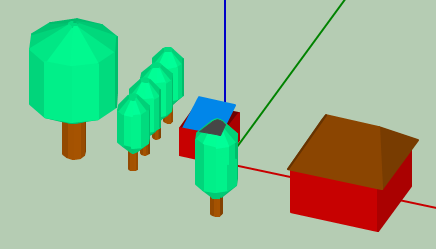
\includegraphics{ivanhoe.png}}
\end{center}
\caption{Ivanhoe system in Denver, CO.}
\label{fig:ivanhoe}
\end{figure}


\begin{figure}[h!]
\begin{center}
\resizebox{3.1in}{!}{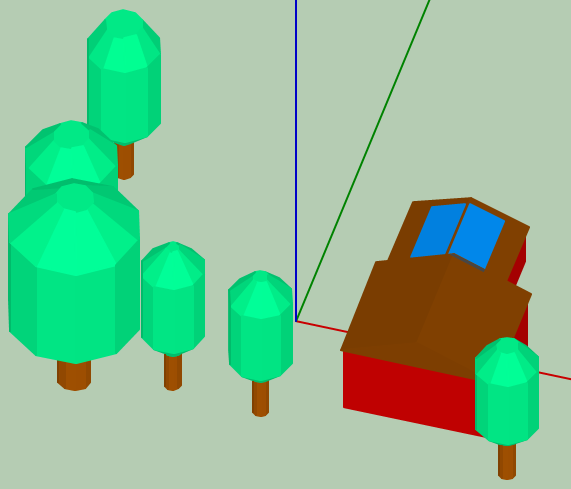
\includegraphics{babbitt.png}}
\end{center}
\caption{Babbitt system in Los Angeles, CA.}
\label{fig:babbitt}
\end{figure}

\begin{figure}[h!]
\begin{center}
\resizebox{3.1in}{!}{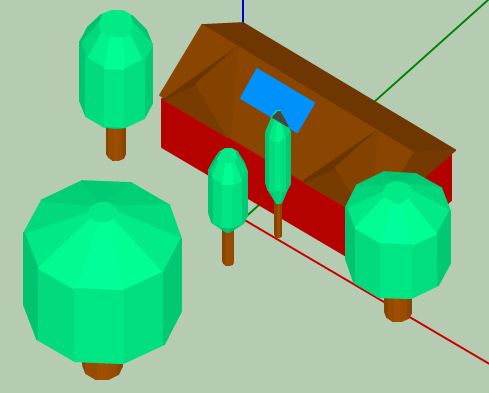
\includegraphics{halsted.png}}
\end{center}
\caption{Halsted system in Los Angeles, CA.}
\label{fig:halsted}
\end{figure}

\begin{figure}[h!]
\begin{center}
\resizebox{3.1in}{!}{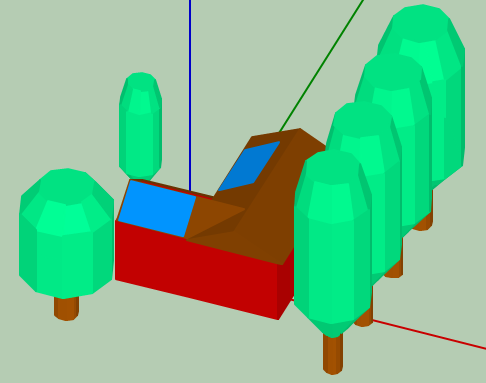
\includegraphics{paradise.png}}
\end{center}
\caption{Paradise system in Soquel, CA.}
\label{fig:paradise}
\end{figure}

\begin{table}[h!]
\begin{center}
\begin{tabular}{lccc}
Scene & SAM & PVsyst & PV*SOL \\
\hline
Ivanhoe & 17.7~\% & ? & ? \\
Babbitt  & 9.3~\% & ? & ? \\
Halsted  & 9.7~\% & ? & ? \\
Paradise & 12.4~\% & ? & ? \\
\end{tabular}
\caption{Sky diffuse loss estimates for real systems.}
\label{tab:diffuse_loss_systems}
\end{center}
\end{table}


\begin{figure*}[h!]
\begin{center}
\scalebox{0.55}{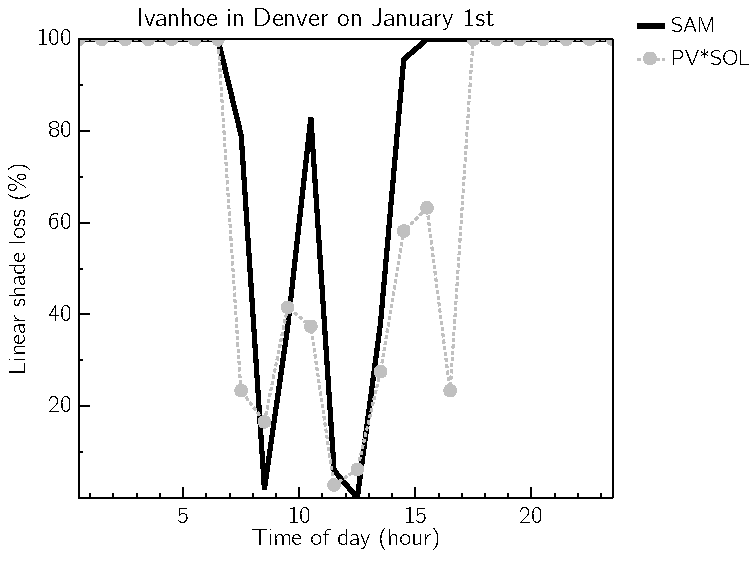
\includegraphics{ivanhoe_in_denver_1.pdf}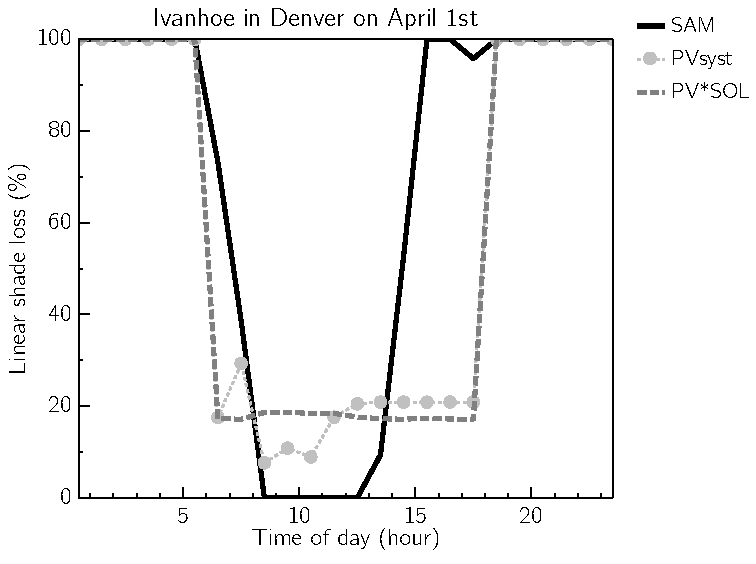
\includegraphics{ivanhoe_in_denver_2.pdf}}
\scalebox{0.55}{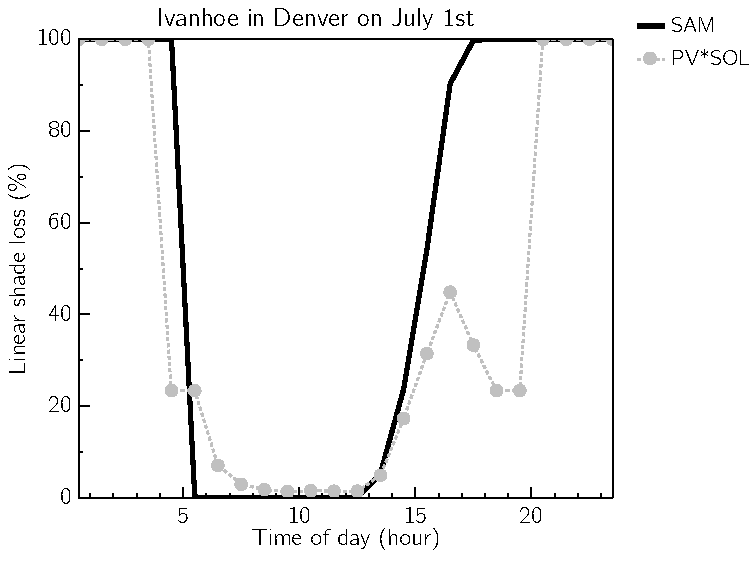
\includegraphics{ivanhoe_in_denver_3.pdf}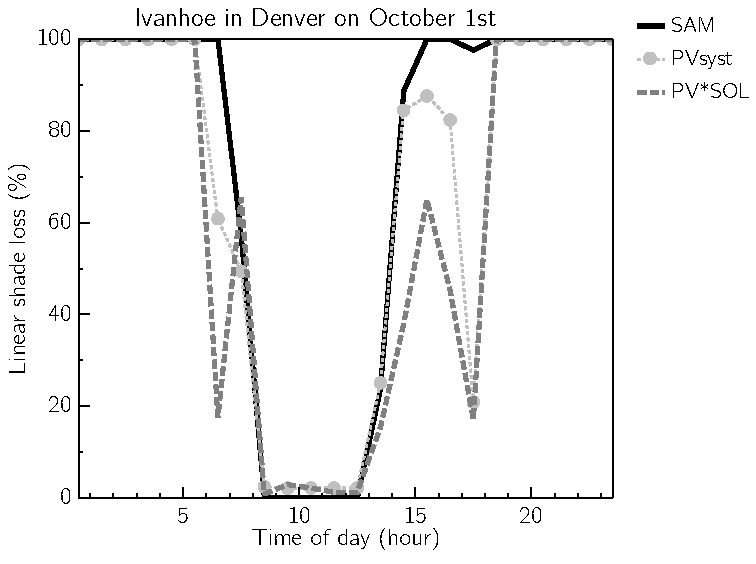
\includegraphics{ivanhoe_in_denver_4.pdf}}
\end{center}
\caption{Daily shade loss profiles for the Ivanhoe system in Denver.}
\label{fig:ivanhoe_denver_profiles}
\end{figure*}


\begin{figure*}[h!]
\begin{center}
\scalebox{0.55}{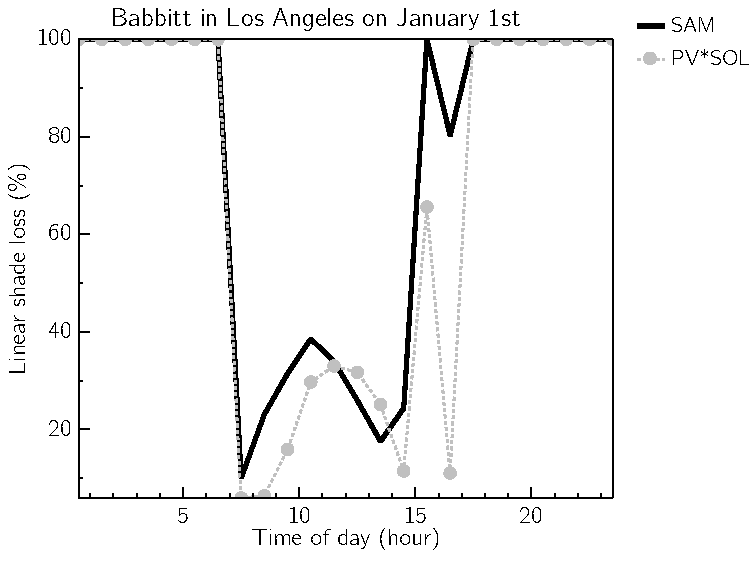
\includegraphics{babbitt_in_los_angeles_1.pdf}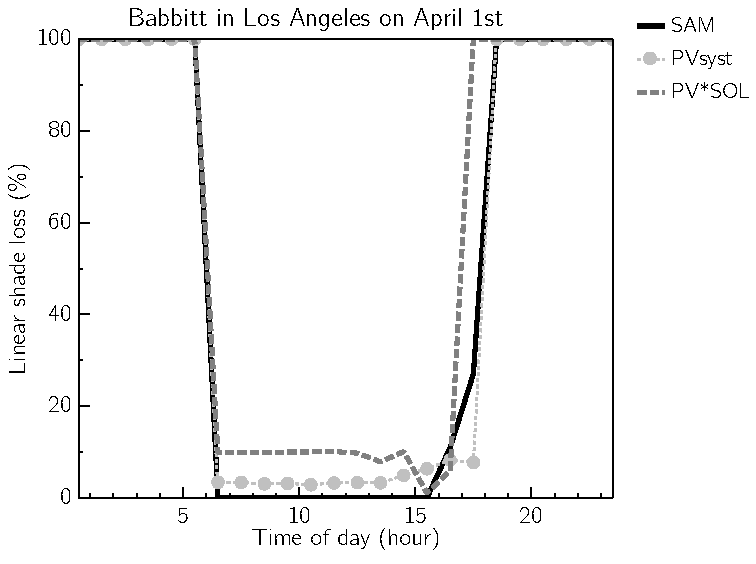
\includegraphics{babbitt_in_los_angeles_2.pdf}}
\scalebox{0.55}{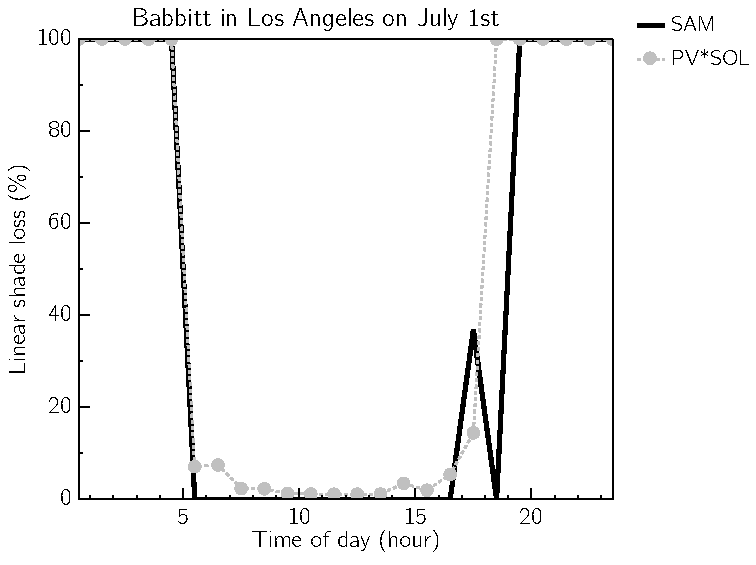
\includegraphics{babbitt_in_los_angeles_3.pdf}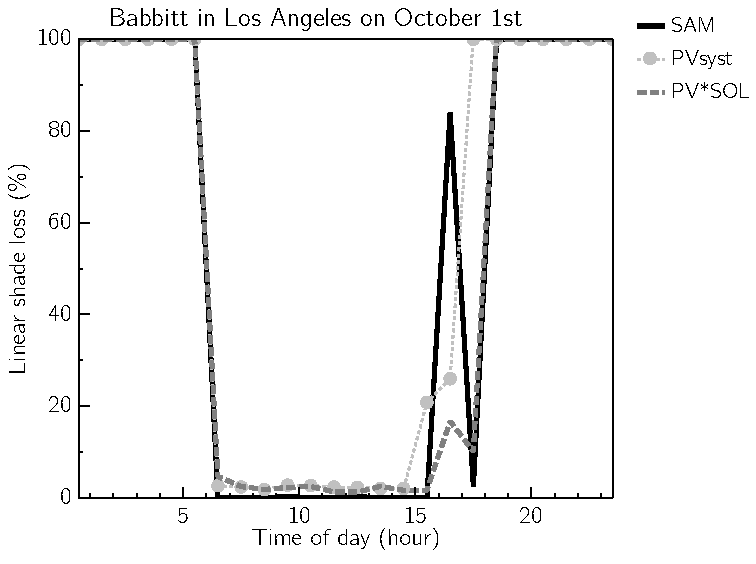
\includegraphics{babbitt_in_los_angeles_4.pdf}}
\end{center}
\caption{Daily shade loss profiles for the Babbitt system in Los Angeles.}
\label{fig:babbitt_los_angeles_profiles}
\end{figure*}


\begin{figure*}[h!]
\begin{center}
\scalebox{0.55}{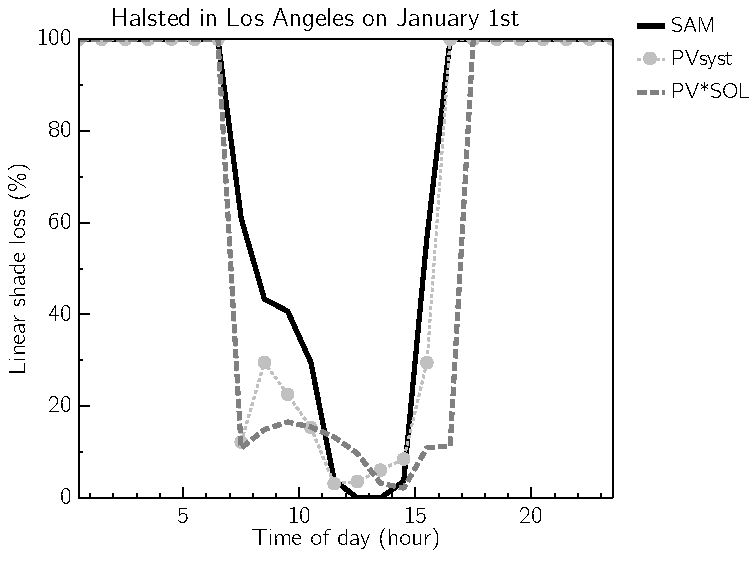
\includegraphics{halsted_in_los_angeles_1.pdf}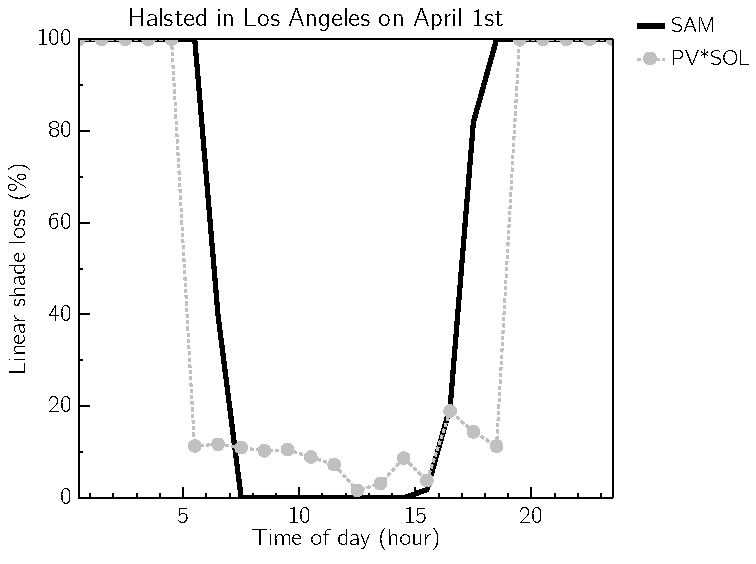
\includegraphics{halsted_in_los_angeles_2.pdf}}
\scalebox{0.55}{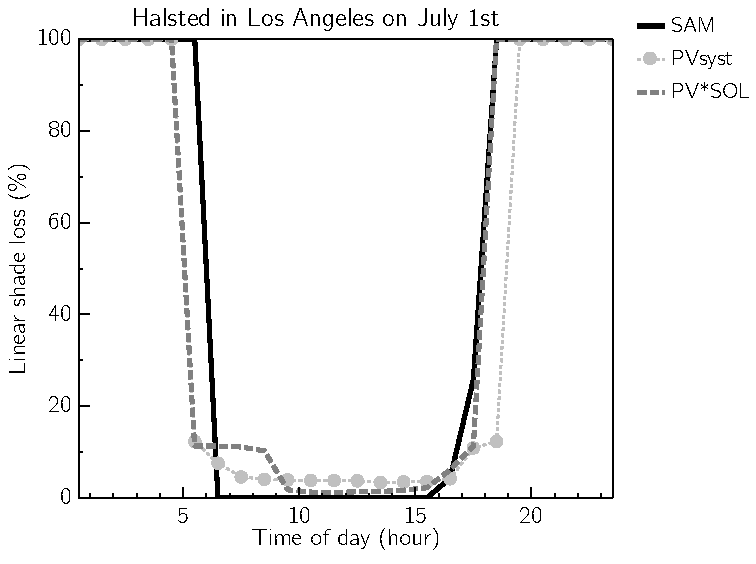
\includegraphics{halsted_in_los_angeles_3.pdf}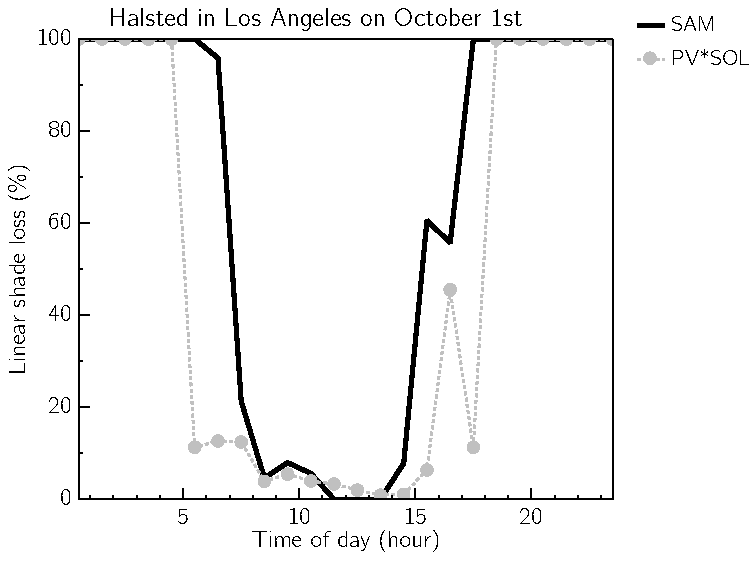
\includegraphics{halsted_in_los_angeles_4.pdf}}
\end{center}
\caption{Daily shade loss profiles for the Halsted system in Los Angeles.}
\label{fig:halsted_los_angeles_profiles}
\end{figure*}




\begin{figure*}[h!]
\begin{center}
\scalebox{0.55}{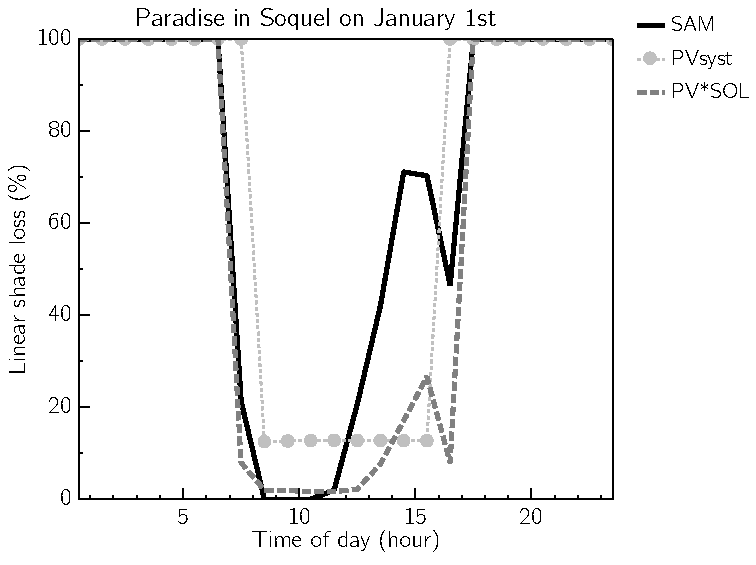
\includegraphics{paradise_in_soquel_1.pdf}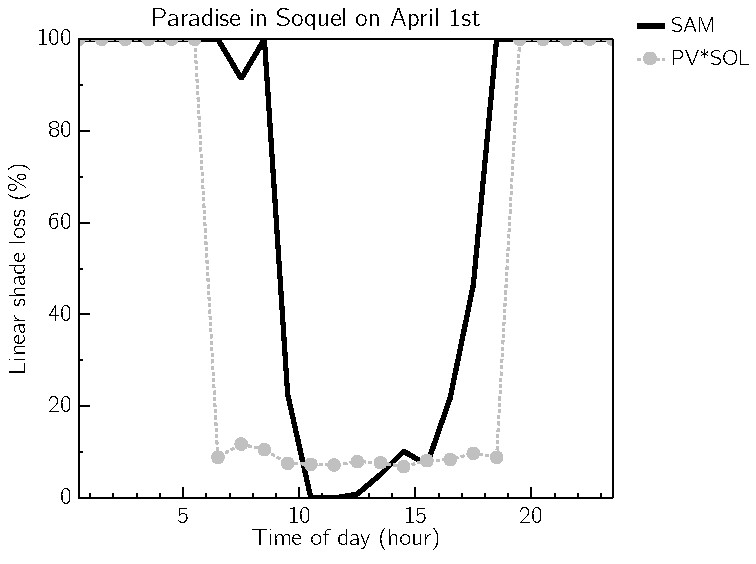
\includegraphics{paradise_in_soquel_2.pdf}}
\scalebox{0.55}{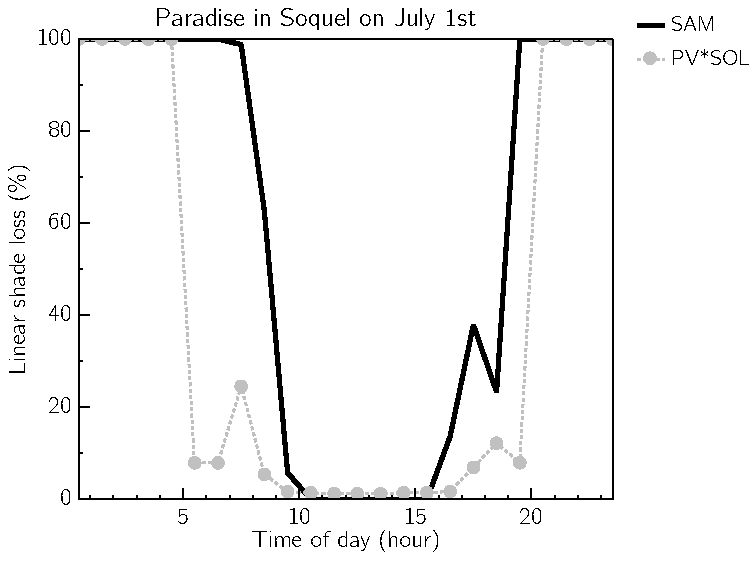
\includegraphics{paradise_in_soquel_3.pdf}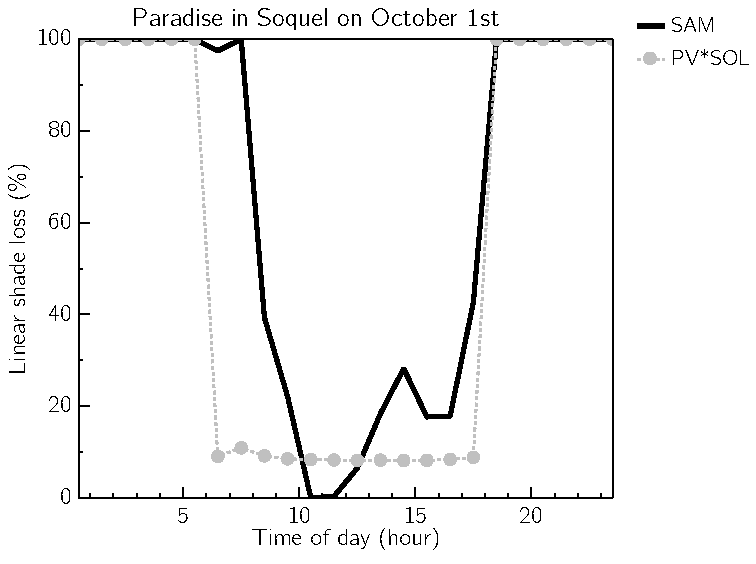
\includegraphics{paradise_in_soquel_4.pdf}}
\end{center}
\caption{Daily shade loss profiles for the Paradise system in Soquel.}
\label{fig:ivanhoe_denver_profiles}
\end{figure*}




\section{Sensitivity to Scene Error}

Lorem ipsum errorum.

\section{Time Step Effects}

Lorem ipsum timestepitum.

\section{Conclusions}

Lorum ipsum conclusionem.


%%%%%%%%%%%%%%%%%%%%%%%%%%%%%%%%%%%%%%%%%%%%%%%%%%%%%%%%%%%%%%%%%%%%%%
\begin{acknowledgment}
This work was supported by the U.S. Department of Energy under Contract No. DE-AC36-08-GO28308 with the National Renewable Energy Laboratory.  We also are immensely grateful to Dr. T. T. Mai for sharing solar access measurements and system specifications for the ``Paradise'' system considered in this report.
\end{acknowledgment}

%%%%%%%%%%%%%%%%%%%%%%%%%%%%%%%%%%%%%%%%%%%%%%%%%%%%%%%%%%%%%%%%%%%%%%
% The bibliography is stored in an external database file
% in the BibTeX format (file_name.bib).  The bibliography is
% created by the following command and it will appear in this
% position in the document. You may, of course, create your
% own bibliography by using thebibliography environment as in
%
% \begin{thebibliography}{12}
% ...
% \bibitem{itemreference} D. E. Knudsen.
% {\em 1966 World Bnus Almanac.}
% {Permafrost Press, Novosibirsk.}
% ...
% \end{thebibliography}

\begin{thebibliography}{8}

\bibitem{suneye} Solmetric SunEye 210 Shade Tool. \url{http://www.solmetric.com/buy210.html}, August 2016.

\bibitem{solarpathfinder} Solar Pathfinder. \url{http://www.solarpathfinder.com}, August 2016.


\bibitem{jakubiec2013} Jakubiec, J; Reinhart C.; \emph{A method for predicting city-wide electricity gains from photovoltaic panels based on LiDAR and GIS data combined with hourly Daysim simulations}. Solar Energy, vol.93, pp.127-143, 2013.

\bibitem{melius2013}  Melius J.; Margolis R.; Ong S.; \emph{Estimating rooftop suitability for PV: a review of methods, patents, and validation techniques}. NREL TP/6A20-60593, 2013.

\bibitem{pvsyst} PVsyst Version 6.47, \url{http://www.pvsyst.com}, August 2016.

\bibitem{pvsol} Valentin Software, PV*SOL Premium Version 2016 R6, \url{http://www.valentin-software.com/en/products/photovoltaics/57/pvsol-premium}, August 2016.

\bibitem{sam} National Renewable Energy Laboratory, \emph{System Advisor Model}, \url{http://sam.nrel.gov}, August 2016.

\bibitem{helioscope} Folsom Labs, \emph{Helioscope}, \url{https://helioscope.folsomlabs.com/}, August 2016.

\bibitem{pvcomplete} PV Complete, \url{http://pvcomplete.com}, August 2016.

\bibitem{blair2013} Blair, N.; Gilman, P.; Dobos, A. P. \emph{Comparison of Photovoltaic models in the System Advisor Model}. American Solar Energy Society, SOLAR 2013 Conference, 2013.

\bibitem{freeman2013} Freeman, J.; Whitmore, J.; Kaffine, L.; Blair, N.; Dobos, A.; \emph{System Advisor Model: Flat Plate Photovoltaic Performance Modeling Validation Report}. NREL/TP-6A20-60204, 2013.

\bibitem{freeman2014} Freeman, J.; Whitmore, J.; Blair, N.; Dobos, A.; \emph{Validation of Multiple Tools for Flat Plate Photovoltaic Modeling Against Measured Data.} 2014 IEEE 40th Photovoltaic Specialist Conference (PVSC), Denver, CO, 2014.

\bibitem{haroon2012} Haroon, S.; \emph{PV Performance and Yield Comparisons, NREL SAM and PVSYST}. Suniva Corporation. Presentation at the SAM Virtual Conference, \url{https://sam.nrel.gov/conferences}, June 2012

\bibitem{yates2010} Yates, T., Hibberd, B., \emph{Production Modeling for GridTied PV Systems}, Solar Pro Magazine, Issue 3.3, April/May 2010. 


%\bibitem{macalpine2015} MacAlpine, S.; Deline, C.; \emph{Simplified Method for Modeling the Impact of Arbitrary Partial Shading Conditions on PV Array Performance}.  Proc. IEEE 41st PVSC Conf, New Orleans, LA, June, 2015.


\end{thebibliography}

\end{document}
